\documentclass{article}

\usepackage[utf8]{inputenc}
\usepackage[frenchb]{babel}
\usepackage[T1]{fontenc}

\usepackage{amsmath}
\usepackage{amssymb}

\usepackage[cm]{fullpage}
\usepackage{multicol}
\usepackage{graphicx}
\usepackage[colorlinks=true, allcolors=black]{hyperref}

\author{Martin Janin}
\title{Modèle 3D d'un objet à partir de photographies: Extraction de silhouette}

\begin{document}

\maketitle

Le travail effectué est celui prévu. La majorité de l'étude a été concentrée sur la détection de contours. La segmentation de l'image obtenue étant effectuée par le procédé simple présenté par Baumgart.

\noindent\makebox[\linewidth]{\rule{\textwidth}{0.4pt}}
\vspace{-0.8cm}
\tableofcontents
\noindent\makebox[\linewidth]{\rule{\textwidth}{0.4pt}}

\bigskip
\bigskip

\section{Introduction}

Le travail consiste en l'implémentation complète d'un script d'extraction de silhouette en python. Celle-ci a entraîné une réflexion importante sur l'optimisation du programme, de la manière d'implémenter les différentes étapes jusqu'au choix des types et structures utilisés.

\pagebreak

\begin{multicols}{2}

\section{Choix d'implémentation}

La totalité du programme est écrite en python. Il comprend certaines commandes en bash afin de suivre l'évolution de l'utilisation de la mémoire vive.

Les modules utilisés sont :

\begin{tabular}{l p{5cm}}
	numpy & $\longrightarrow$ structure et opérations \\
	system & $\longrightarrow$ suivie de la mémoire \\
	matplotlib & $\longrightarrow$ tracé et affichage des images \\
	itertools & $\longrightarrow$ outils sur les générateurs \\
	time & $\longrightarrow$ suivi du temps d'execution de chaque étape
\end{tabular}

\subsection{Types et structures}

Le programme prend en entrée une image RGB de taille de l'ordre du mégapixel. Traiter des données de cette taille motive des choix qui ne sont pas habituels dans d'autres domaines de l'informatique.

\subsubsection{Type}
Le type retenu est le type float32 de numpy, conjugué naturellement au type complex64. C'est le meilleur choix pour plusieurs raisons :
\begin{itemize}
	\item Les opérations sur les flottants sont plus rapides que sur les entiers. En effet, les processeurs sont d'abord conçus pour effectuer des opérations sur des nombres flottants.
	\item Les 8 bits alloués à l'exposant du type float32 permettent un nombre maximal de $10^{256}$ ce qui évite tout dépassement de capacité.
	\item Il est bien plus aisé de normaliser une image de flottants puisque le type gère de lui même la perte de précision (contrairement aux entiers)
	\item Du fait des grandes complexités spatiales, il était impossible d'utiliser des flottants sur 64bits.
\end{itemize}

\subsubsection{Structure}
En ce qui concerne la structure adoptée, il s'agit des tableaux numpy, pour des raisons d'efficacité. On est amené à utiliser des tableaux à 5 dimensions, réparties comme suit :
\begin{itemize}
	\item Les 3\up{ème} et 4\up{ème} correspondent au plan de l'image : indexer par rapport à ces dimensions correspond à choisir un pixel.
	\item Les deux premières dimensions correspondent au voisinage de chaque pixel. Chaque pixel contient en effet tout son voisinage afin de pouvoir effectuer des opérations dessus.
	\item La 5\up{ème} dimension est celle des composantes. On manipulera en effet des images composites, à l'instar d'une image RGB, ce qui permet d'effectuer les mêmes opérations sur toutes les composantes simultanément.
\end{itemize}

\subsection{Complexité}

Les choix d'implémentation ont principalement été motivés par l'optimisation de la complexité.

\subsubsection{Complexité temporelle} 
En théorie, la meilleure manière d'effectuer des opérations sur plusieurs millions de pixels est de vectoriser les calculs, c'est-à-dire d'effectuer les calculs simultanément. On utilise pour cela des GPU (Graphical Process Unit) dont les circuits sont conçus pour effectuer simultanément des opérations sur des vecteurs. Cependant, programmer de manière efficace sur GPU nécessite une maitrise de languages de bas niveau conçus spécialement pour. En pratique, les calculs vectoriels ont donc été faits avec numpy. Bien que numpy utilise uniquement le CPU pour toutes les opérations, quand les calculs sont correctement vectorisés, ils sont effectués par des boucles sous-jacentes codées en C. Les opérations vectorielles de numpy sont significativement plus rapides qu'en python et simule donc bien le comportement de calculs vectorisés.

\subsubsection{Complexité spatiale}
Vectoriser les calculs nécessite cependant de stocker simultanément les variables intermédiaires de millions de calculs dans la mémoire vive. Il en résulte une grande complexité spatiale. En effet, effectuer un calcul sur le voisinage de chaque pixel demande : $\mathtt{TailleDesDonnées} \times \mathtt{TailleDuVoisinage} \times \mathtt{TailleDeLimage} \times \mathtt{NombreDeComposantes}$ ce qui dans l'implémentation proposée est parfois de l'ordre de :  $8 \mathtt{Octet} \times 500 \time 10 \mathtt{Mpix} \times 10$ soit 4Gio. Les ordinateurs actuels disposent d'une mémoire de l'ordre de 5Gio. L'optimisation spatiale est donc également importante. Comme il n'y a aucun moyen de gérer explicitement la mémoire en python, la solution mise en oeuvre a consisté à coder les fonctions clés de sorte que le calcul se face en place autant que possible.

\subsubsection{Coût de copie}
Il faut noter enfin, que lorsqu'il s'agit d'effectuer des opérations sur le voisinage de chaque pixel, il est nécessaire de copier un grand nombre de fois l'image en mémoire (cf. structure). Le coût temporel de ces copies est non négligeable même avec l'optimisation sous-jacente de numpy. Cependant, au moyen d'une manipulation bas niveau des mémoires de travail vectorielles (registres vectoriels) d'un GPU, il serait possible de rendre ces coûts de copie négligeables.

\section{Procédé et Résultats}

On prend pour exemple l'image ci-dessous.
\begin{figure*}
	\centering
	\raisebox{-0.5\height}{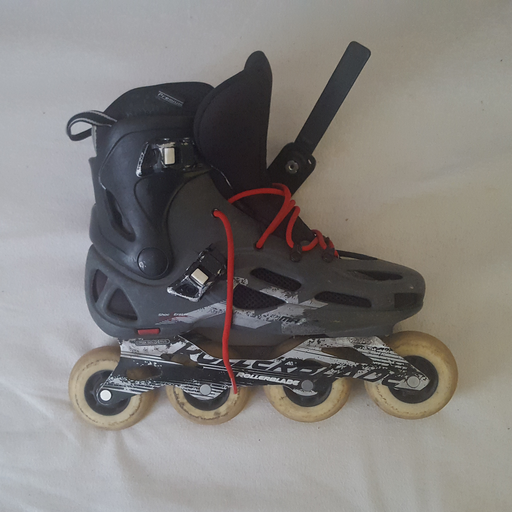
\includegraphics[height=3cm]{images/roller.png}}
\end{figure*}
Détaillons les différentes étapes de ce procédé. Les différentes étapes ainsi que leurs résultats sont résumé dans un \hyperref[tab]{tableau en fin de document}

\subsection{Convertion dans l'espace LAB}

L'espace LAB est un espace colorimétrique standardisé qui a pour but d'offir une représentation plus proche de la vision humaine. Elle est construite sur trois composante :
\begin{itemize}
	\item L : représente l'intensité lumineuse. C'est la moyenne des composantes RGB
	\item A et B : décrivent la couleur. Ce sont respectivement les différences G - R et G - B
\end{itemize}
La norme LAB définit ces trois composantes comme les moyennes et différences ci-dessus auquelles sont appliquées des transformations non linéaires complexes. Ces transformations sont dépendantes de la machine. Cependant l'objectif ici n'est pas de s'approcher de la vision humaine mais de produire une image dont l'analyse produira de meilleurs résultats. Ces transformations ont donc été abandonnées et les composantes LAB ont été calculées par simple différences et moyennes.

La complexité de cette conversion est $\theta(\nu(n^2))$ où n est la largeur de l'image (supposée carrée).

\subsection{1\up{er} Filtrage - Domaine fréquentiel - Calcul des composantes de texture}

En plus de l'intensité et de la couleur, un bon indicateur de l'appartenance d'un pixel à un objet est sa texture. On entend par là l'éventuelle répetition périodique d'un motif. On mesure la valeur de texture d'un pixel relative à un motif en effectuant le produit de convolution du voisinage de ce pixel avec le motif en question, et en sommant la réponse obtenue.

On rappel la définition du produit de convolution. 
Soient f et g deux signaux d'extension finie.
$$ f * g : x \rightarrow \int_{-\infty}^{+\infty} f(t-x) \cdot g(t) \mathrm dt $$
Dans sa version discrète, avec u et v deux signaux discrets d'extension finie :
$$ u * v : n \rightarrow \sum_{k \in \mathbb{Z}} u(k -n) \cdot v(k)$$
Que l'on peut étendre à des signaux discrets de dimension 2 (des images):
$$ u * v : (n, m) \rightarrow \sum_{(k,l) \in \mathbb{Z}^2} u(k - n, l - m) \cdot v(k, l)$$
On définit alors la réponse d'une image I à un motif M par :
$$\mathtt{texture}_M : (i, j) \rightarrow \sum_{(k,l) \in \mathbb{Z}^2} (V(i, j) * M)(k, l)$$
Où $V((i, j)$ désigne un voisinage du pixel $(i, j)$ dans l'image $I$.

Afin de calculer plus efficacement ces produits de convolution, on utilise la transformée de fourier discrète. En effet, une proprité de cette opérateur que nous noterons $DF$ est:
$$u * v = DF^{-1}(DF(u) \cdot DF(v))$$
Comme on va réaliser de nombreux produits de convolution, l'idée est de calculer la transformée de fourier discrète du voisinage de chaque pixel et de réaliser ensuite une simple multiplication par la transformée de Fourier du motif. Afin d'accélérer encore les calculs, on utilise l'algorythme de transformée de Fourier rapide. >>>Voir annexe<<<. La complexité atteinte de la transformée de Fourier de chaque voisinage de l'image est $\theta(log_2(t) \cdot \nu(t^2 \cdot n^2))$ où $t$ est la taille des voisinages.

On choisit ensuite de multiplier la transformée de fourier de chaque voisinage par des filtres gaussiens, représentant des motifs de base dans le domaine fréquentiel. Chaque filtrage produit une nouvelle composante de l'image que l'on rajoute à l'image de départ.

\subsection{2\up{ème} Filtrage - Domaine spatial - Détection des bordures}

Il s'agit ensuite de filtrer les composantes de l'images afin d'en extraire les bordures. Le principe est de remplacer la valeur de chaque pixel par une somme pondérée des pixels de son voisinage. J. Canny a montré que le filtre (i.e. les coefficients de la somme) optimal pour différencier les pas d'intensité du reste de l'image est en bonne approximation la dérivée d'une fonction gaussienne. On obtient après filtrage de chacune des composantes dans de multiples directions les bordures correspondant à chacune d'entre elle. Tous les calculs pouvant être correctement vectorisés, la complexité totale de l'opération est : $\theta(t^2 \cdot \nu(n^2 \cdot x))$ où $c$ est le nombre de composantes de l'image.

\subsection{Lissage parabolique}

Cependant, les bordures obtenues tendent à avoir une extension spatiale importante et des bordures issues des composantes de texture, on observe des bordures doublées par rapport à l'image initiale. Ces doubles bordures s'explique par l'extension spatiale du filtrage fréquentiel donnant lieux aux composantes de texture. On a alors recourt à un lissage parabolique.

Pour chaque direction de filtrage, on approxime le voisinage de chaque pixel par un cylindre parabolique d'axe cette direction. On remplace alors la valeur du pixel par :
$$\frac{c}{\text{distance au max local}} = \frac{c^+}{\left(\frac{|b|}{2a^+}\right)}$$
Cette opération permet d'affiner les bordures et de supprimer les doubles bordures.

\subsection{Sommation des composantes}

On obtient à la suite de ces opérations de nombreuses composantes :
\begin{itemize}
	\item Pour les composantes de texture $3\mathtt{couleur} + 3\mathtt{couleur} \times 4\mathtt{écarttype} = 15\mathtt{composante}$
	\item Pour le filtrage $15\mathtt{composante} \times 2\mathtt{ecarttype} = 30\mathtt{composante}$
\end{itemize}
Pour obtenir l'image de bordure finale, on réalise une somme pondérée de toutes ces composantes. L'approche idéale consiste à déterminer les coefficients de sommation  par apprentissage supervisé. Dans notre cas, le choix est une conjonction d'empirisme et de valeurs tirées de la littérature.

\subsection{Seuillage}

L'image est seuillée pour obtenir une image binaire. Le seuil de 0.3 (Pour une image préalablement normalisée à 1) est une choix empirique

\subsection{Opérations topologiques}

Afin d'améliorer l'image binaire obtenue, on réalise des opérations topologiques simples. On note \texttt{I} L'ensemble des pixel de valeur 1 dans l'image binaire. On définit alors les opérations suivantes, prenant en paramètre un ensemble \texttt{U} :
\begin{itemize}
	\item Dilatation par \texttt{U}: $\mathcal{D}_\mathtt{U}(\mathtt{I}) = \{p \, | \, \exists q \in \mathtt{I}, \, {p-q} \in \mathtt{U}\}$
	\item Erosion par \texttt{U}: $\mathcal{E}_\mathtt{U}(\mathtt{I}) = \{p \, | \, \forall v \in \mathtt{U}, \, {p+v} \in \mathtt{I}\}$
	\item Fermeture par \texttt{U} : $\mathcal{F}_\mathtt{U} = \mathcal{D}_\mathtt{U} \circ \mathcal{E}_\mathtt{U}$
\end{itemize}
On réalise alors, les opérations suivantes sur l'image binaire :\\
Une érosion par :\\
\medskip
\begin{tabular}{|l|c|r|}
	\hline
	0 & 1 & 0 \\ \hline
	1 & 1 & 1 \\ \hline
	0 & 1 & 0 \\
	\hline
\end{tabular}\\
\medskip
Séquentiellement, des fermetures par:\\
\medskip
\begin{tabular}{|l|c|c|c|r|}
	\hline
	0 & 0 & 0 & 0 & 0 \\ \hline
	0 & 0 & 0 & 0 & 0 \\ \hline
	1 & 1 & 1 & 1 & 1 \\ \hline
	0 & 0 & 0 & 0 & 0 \\ \hline
	0 & 0 & 0 & 0 & 0 \\
	\hline
\end{tabular}\\
\medskip
Auquel on applique des rotations dans 8 directions différentes.

\subsection{Approximation polygonale}

On extrait d'abord le contour extérieur de l'image obtenue en partant du point le plus haut et en se déplaçant de pixel en pixel. On attribut des priorité aux directions de déplacement afin de parcourir effectivement le contour extérieur dans le sens trigonométrique. Par exemple si le sens de déplacement courant est \texttt{Bas}, on appliquera comme ordre de priorité : \texttt{Gauche - Bas - Droite - Haut}.
Une fois ce contour obtenu, on cherche à l'approximer par un polygone de tel sorte que la distance maximale entre le contour et le polygone soit inférieure à un seuil donné. Pour celà, on initialise le polygone par un segment alant du point le plus haut au point le plus bas puis on itère le procédé suivant sur chaque segment :
\begin{itemize}
	\item On calcul $D$ la distance maximale du segment au contour
	\item Si $D > \mathtt{seuil}$ on coupe le segment en deux en ajoutant au polygone le point le plus éloigné du segment.
\end{itemize}

\section{Conclusion}
	Le résultat obtenu, bien qu'imprécis permet ensuite, en combinant les silhouettes obtenues de plusieurs points de vues, de reconstituer le modèle 3D de l'objet. On a vu comment numpy pouvait permettre par la vectorisation (virtuelle), d'effectuer des opérations complexes sur des millions de données. L'optimisation spatiale et temporelle rigoureuse permet de mener à bien des calculs complexes (transformée de Fourier) en un temps raisonnable ($\approx 45s$)

\end{multicols}

\begin{figure}
\newcommand{\tabinc}[2] {
	\smash{\raisebox{-1\height}{\includegraphics[height=#1]{#2}}}\vspace{#1}
	}

\noindent\begin{tabular}{|c|p{0.125\textwidth}|p{0.5\textwidth}|p{0.1\textwidth}|p{0.125\textwidth}|}
	\hline
	& Opération & Description & Paramètres & Resultats \\ 
	\hline
		1 & Convertion espace LAB 
		& \vspace{0.01cm}$(L = \frac{R + G + B}{2})$ code l'intensité, $(A = \frac{G - R + 1}{2})$ et $(B = \frac{G - B + 1}{2})$ la couleur. Cette espace est 	plus relevant pour détecter les bordures d'objet. 
		& 
		& \tabinc{2cm}{images/roller_lab.jpg} \\ 
	\hline
		2 & Calcul des composantes de texture 
		& On réalise la convolution du voisinage de chaque pixel par une gaussienne d'orientation et d'écart type variables. On calcul pour cela la transformée de Fourier de chaque voisinage 
		& $\sigma = 4$ \;\;\;\;\;\;\;\; 4 directions
		& \tabinc{2cm}{images/roller_respn.jpg} \\ 
	\hline
		3 & Filtrage 
		& On filtre toutes les composantes par des filtres de Canny (dérivée d'une gaussienne) d'orientation et d'écart type variables. 
		& $\sigma \in \{1,2\}$, 8 directions 
		& \tabinc{2cm}{images/roller_filteredn.jpg} \\ 
	\hline
		4 & Lissage parabolique 
		& On approxime le voisinage de chaque pixel par une parabole $(ax^2 + bx + c)$ par la méthode des moindres carrés. On remplace l'image par l'image lissée : $$I = \frac{c^+}{\text{distance au max local}} = c^+ \cdot \frac{2a^+}{|b|}$$ 
		& 8 directions 
		& \tabinc{2cm}{images/roller_localisedn.jpg}\\ 
	\hline
		5 & Sommation des réponses 
		& On somme les 20 composantes obtenues $[(2 \text{couleurs} + 4 \text{orientation} * 2 \text{couleurs}) * 2 \text{écart type}]$ en les pondérants par des coefficients piochés dans la littérature. 
		& coefficients de sommations 
		& \tabinc{2cm}{images/roller_resn.jpg} \\ 
	\hline
		6 & Seuillage 
		& On seuille l'image pour obtenir une image binaire 
		& $\text{seuil} = 0.2$ 
		& \tabinc{2cm}{images/roller_binn.jpg} \\ 
	\hline
		7 & Opérations topologiques 
		& On érode (tous les pixels non entourés sont supprimés) puis on dilate (tous les voisins des pixels sont allumés) successivement afin de fermer le contour de l'image 
		& filtres de fermeture 
		& \tabinc{2cm}{images/roller_closedbinn.jpg} \\ 
	\hline
		8 & Approximation polygonale 
		& On approxime le contour extérieur de l'objet par un polygone en séparant récursivement les segments d'un polygone jusqu'a atteindre un seuil d'approximation (distance maximale polygone-contour) 
		& seuille d'approximation : 10 pixels 
		& \\
	\hline
\end{tabular}
\caption{Tableau Récapitulatif}
	\label{tab}
\end{figure}

\end{document}
